\chapter{Experiments}
\label{chap:experiments}

This chapter reports the $2\times2$ backbone-by-language ablation defined in
Section~\ref{ablation}, evaluated entirely in live MineRL rollouts. I first fix
the evaluation setup and a random-policy sanity floor
(Section~\ref{sec:exp-setup}), then present the two findings the design is built
to deliver: whether the language prompt measurably reshapes the policy
(Section~\ref{sec:exp-cond}), and how much of the demonstrated task each cell
actually completes (Section~\ref{sec:exp-task}). I then contrast these rollout
outcomes with the held-out frame metrics (Section~\ref{sec:exp-offline}), which
tell a strikingly different story. A final probe
(Section~\ref{sec:exp-film}) asks whether the weaker backbone fails because its
features are uninformative or because the head cannot read them. Throughout, I
treat the online rollout statistics of Section~\ref{sec:rollout} as primary and
report per-step firing rates from the recorded \texttt{steps} logs rather than
the per-step dominant-action summary, which undercounts simultaneously held
keys.

\section{Experimental Setup}
\label{sec:exp-setup}

The four cells are the knob-free trajectory-split checkpoints
$\{\text{LLaVA},\text{CLIP}\}\times\{\text{lang},\text{nolang}\}$ of
Section~\ref{ablation}: Exp~1 (LLaVA + prompt), Exp~2 (CLIP + prompt), Exp~3
(LLaVA, no prompt) and Exp~4 (CLIP, no prompt). Every cell is evaluated under
four conditions that vary only the environment and the prompt string, holding
the decode (Section~\ref{sec:rollout}) and the base seed fixed:

\begin{table}[ht]
\centering
\begin{tabular}{llll}
\hline
Condition & Environment & Prompt & Probes \\
\hline
A (\texttt{chop\_nocap}) & \texttt{ChopATree640Fast} & \enquote{} (empty)       & off-task floor \\
B (\texttt{chop\_ood})   & \texttt{ChopATree640Fast} & \enquote{Play Minecraft.} & out-of-task prompt \\
C (\texttt{chop\_task})  & \texttt{ChopATree640Fast} & \enquote{chop a tree}     & on-task prompt \\
D (\texttt{dirt\_task})  & \texttt{CollectDirt640Fast} & \enquote{collect dirt}  & second task \\
\hline
\end{tabular}
\caption{The four rollout conditions. Conditions A--C share the chop
environment and vary only the prompt, isolating the prompt's effect on
behaviour; D evaluates a second task. Each cell is run for $10$ episodes of
$1000$ steps per condition at base seed $0$.}
\label{tab:conditions}
\end{table}

Comparing conditions A, B and C within a single cell isolates the effect of the
prompt, since the environment, the seed and the decoder are identical and only
the conditioning string changes. I quantify each binary key's firing rate per
condition with a Wilson $95\%$ confidence interval, compare conditions with a
two-proportion $z$-test, and report Cohen's $h$ as an effect size, exactly as
described in Section~\ref{sec:rollout}. Because each condition contributes
roughly $10^4$ steps, the per-step intervals are tight and even small rate
differences reach nominal significance; I therefore lean on the effect size and
on the random floor below, not on the $p$-value alone, to separate a meaningful
shift from a merely detectable one.

\paragraph{Random-policy floor.} To confirm that the trained agents act rather
than twitch, I run a random policy in the same environments at the same seed:
each binary key is flipped independently with probability $0.1$ and each camera
axis is drawn uniformly from $[-5^\circ,5^\circ]$, with no model in the loop.
The random policy fires every key at $9.6$--$10.5\%$ of steps, moves the camera
by $2.5^\circ$ on average, and collects \emph{zero} logs and \emph{zero} dirt
across all $20$ episodes. This is the chance baseline against which the trained
cells are read: Figure~\ref{fig:profile} shows every trained cell concentrating
its mass on \texttt{attack} and \texttt{forward} far above the flat $\sim\!10\%$
random line, confirming the policies diverge from chance before any
prompt-conditioning question is asked.

\begin{figure}[ht]
\centering
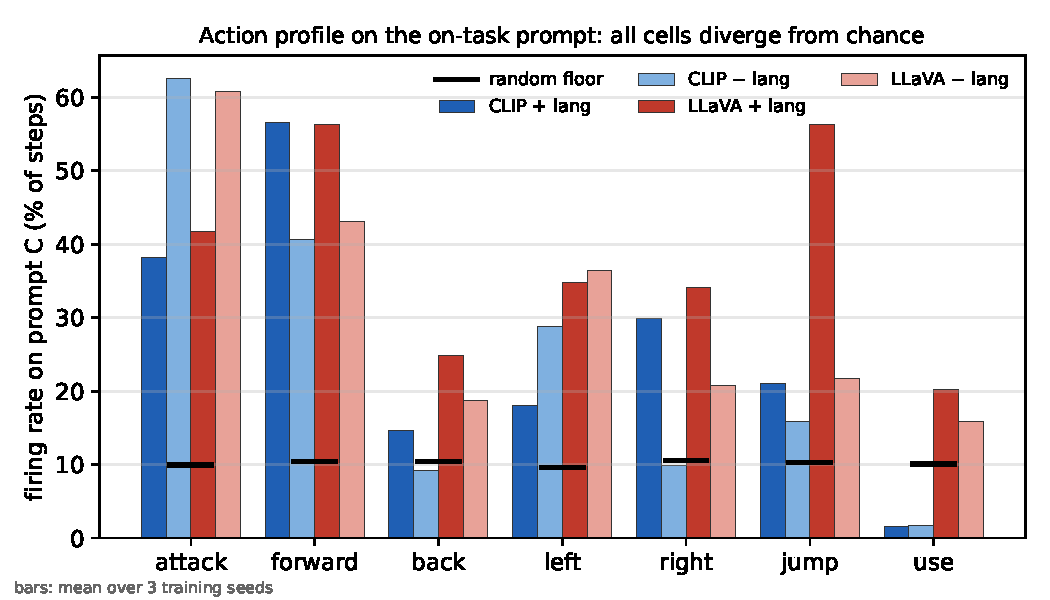
\includegraphics[width=0.92\textwidth]{figures/fig_action_profile.pdf}
\caption{Per-key firing rate on the on-task prompt (condition C) for the four
cells, against the random-policy floor (black ticks). All four trained cells
place most of their mass on \texttt{attack} and \texttt{forward}, several times
the $\sim\!10\%$ chance rate, so none is behaving randomly; they
differ in \emph{how} that mass is distributed.}
\label{fig:profile}
\end{figure}

\section{Language Conditioning}
\label{sec:exp-cond}

The central question of the prompt ablation is whether the language string
changes what the agent does. Table~\ref{tab:conditioning} reports the
\texttt{attack} and \texttt{forward} firing rates across the three chop-prompt
conditions, and Figure~\ref{fig:conditioning} plots the \texttt{attack} channel,
the most discriminative key.

\begin{table}[ht]
\centering
\begin{tabular}{llrrrrr}
\hline
Cell & Key & A (\%) & B (\%) & C (\%) & $\Delta_{\text{C}-\text{A}}$ (pp) & $h$ \\
\hline
Exp~2 CLIP + lang   & attack  & 84.9 & 76.7 & 37.0 & $-48.0$ & $-1.04$ \\
                    & forward & 76.3 & 71.2 & 62.6 & $-13.7$ & $-0.30$ \\
Exp~4 CLIP $-$ lang & attack  & 57.8 & 57.8 & 64.0 & $+6.1$  & $+0.13$ \\
                    & forward & 43.9 & 42.8 & 35.5 & $-8.4$  & $-0.17$ \\
Exp~1 LLaVA + lang  & attack  & 34.9 & 32.6 & 29.8 & $-5.1$  & $-0.11$ \\
                    & forward & 23.9 & 24.5 & 24.1 & $+0.2$  & $+0.00$ \\
Exp~3 LLaVA $-$ lang& attack  & 54.4 & 51.5 & 50.2 & $-4.2$  & $-0.09$ \\
                    & forward & 52.7 & 53.8 & 55.3 & $+2.6$  & $+0.05$ \\
\hline
\end{tabular}
\caption{Firing rates across the three chop-prompt conditions. $\Delta_{\text{C}
-\text{A}}$ is the on-task-minus-empty-prompt change in percentage points and
$h$ is Cohen's $h$ for that pair. Only CLIP + lang shows a large shift
($|h|>0.5$); the other three cells stay within $|h|\le0.17$, the same band as
the no-prompt controls.}
\label{tab:conditioning}
\end{table}

\begin{figure}[ht]
\centering
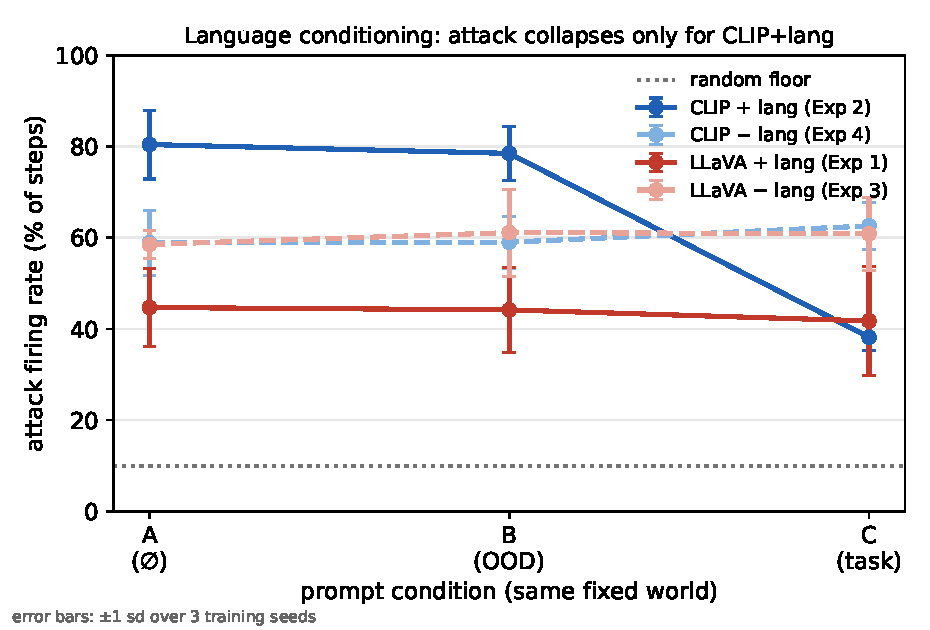
\includegraphics[width=0.82\textwidth]{figures/fig_conditioning.pdf}
\caption{\texttt{attack} firing rate across the empty (A), out-of-task (B) and
on-task (C) prompts; error bars are Wilson $95\%$ intervals (smaller than the
markers). Only CLIP + lang (solid blue) shifts with the prompt, its \texttt{attack}
rate moving from $84.9\%$ to $37.0\%$; the other three cells are flat, and all
sit well above the random floor (dotted).}
\label{fig:conditioning}
\end{figure}

The effect is large and concentrated in a single cell. \textbf{CLIP + lang}
suppresses its \texttt{attack} key from $84.9\%$ under the empty prompt to
$37.0\%$ under \enquote{chop a tree}, a $48$~percentage-point shift with
$h=-1.04$ --- a large effect by any threshold, and the prompt is the only
deliberately varied factor across the two conditions; with $\sim\!10^4$ steps per
condition the per-step intervals are far tighter than this shift, so it cannot be
attributed to rollout noise. The shift is not confined to one key: in the same
cell \texttt{sprint} falls by $29$~pp and rightward steering rises by $18$~pp
alongside the \texttt{forward} drop ($-13.7$~pp), whereas no other cell moves any
channel by more than about $6$~pp. The on-task prompt reorganises the whole
action distribution rather than nudging a single key. \textbf{CLIP $-$ lang}, the same
backbone with the text branch zeroed, is flat: \texttt{attack} moves by
$+6.1$~pp ($h=+0.13$), within the noise band, which is exactly the negative
control the design demands --- when language is removed from the representation,
the prompt string can no longer act.

Both LLaVA cells are flat in both conditions. \textbf{LLaVA + lang} shifts
\texttt{attack} by only $-5.1$~pp ($h=-0.11$) and \texttt{forward} not at all,
and \textbf{LLaVA $-$ lang} is indistinguishable from it ($-4.2$~pp). These
residual shifts reach nominal significance only because each rate is estimated
from $10^4$ steps; their effect sizes ($|h|<0.12$) sit inside the same band as
the no-prompt controls, so they carry no behavioural meaning. The asymmetry
noted in Section~\ref{ablation} sharpens rather than weakens this reading: in
the LLaVA no-prompt cell the prompt still passes through the decoder and only
the pooled text vector is zeroed, so the pooled image features remain
prompt-conditioned --- yet even with that residual pathway, and even with the
explicit text vector present in the prompt cell, LLaVA never separates from its
own control. The defensible conclusion is therefore a statement about the
backbone, not about language in general: \emph{under this frozen-feature regime
the contrastive CLIP text encoder yields a conditioning signal the head uses,
whereas the frozen LLaVA-1.5 backbone does not} --- and, as the probe of
Section~\ref{sec:exp-probe} shows, not because the prompt is absent from its
features but because the pooled representation does not expose it as an axis a
small head can act on.

\section{Task Performance}
\label{sec:exp-task}

Conditioning shows that a prompt changes behaviour; it does not show that the
behaviour completes the task. For task progress I use the reward-independent
peak-inventory measure of Section~\ref{sec:rollout}, the maximum count of the
goal item held during an episode. Chopping is at the floor for every cell ---
no cell collects more than a single log in any episode, in line with the broken
chop reward handler discussed in Section~\ref{sec:rollout} --- so the chop
conditions do not separate the models and I report dirt collection (condition D)
as the discriminating task. Table~\ref{tab:task} and Figure~\ref{fig:task} give
the per-episode results.

\begin{table}[ht]
\centering
\begin{tabular}{lrrrr}
\hline
Cell & dirt$_{\text{A}}$ (chop) & dirt$_{\text{D}}$ (dirt) & $95\%$ CI$_{\text{D}}$ & success$_{\text{D}}$ \\
\hline
Exp~2 CLIP + lang    & 0.8 & 4.30 & $[2.70,\,6.20]$ & $100\%$ \\
Exp~4 CLIP $-$ lang  & 2.5 & 2.30 & $[1.00,\,3.90]$ & $80\%$ \\
Exp~1 LLaVA + lang   & 0.0 & 0.00 & $[0.00,\,0.00]$ & $0\%$ \\
Exp~3 LLaVA $-$ lang & 0.9 & 0.10 & $[0.00,\,0.30]$ & $10\%$ \\
\hline
random policy        & 0.0 & 0.00 & --- & $0\%$ \\
\hline
\end{tabular}
\caption{Dirt collected per episode (mean peak inventory over $10$ episodes).
dirt$_{\text{A}}$ is \emph{incidental} digging in the chop environment under the
empty prompt; dirt$_{\text{D}}$ is digging in the dirt environment under the
on-task prompt. The interval is a $20{,}000$-resample percentile bootstrap of the
dirt$_{\text{D}}$ mean; success is the fraction of episodes collecting any dirt.
The dirt$_{\text{A}}$-versus-dirt$_{\text{D}}$ contrast separates goal-directed
digging from incidental terrain-attacking (see text).}
\label{tab:task}
\end{table}

\begin{figure}[ht]
\centering
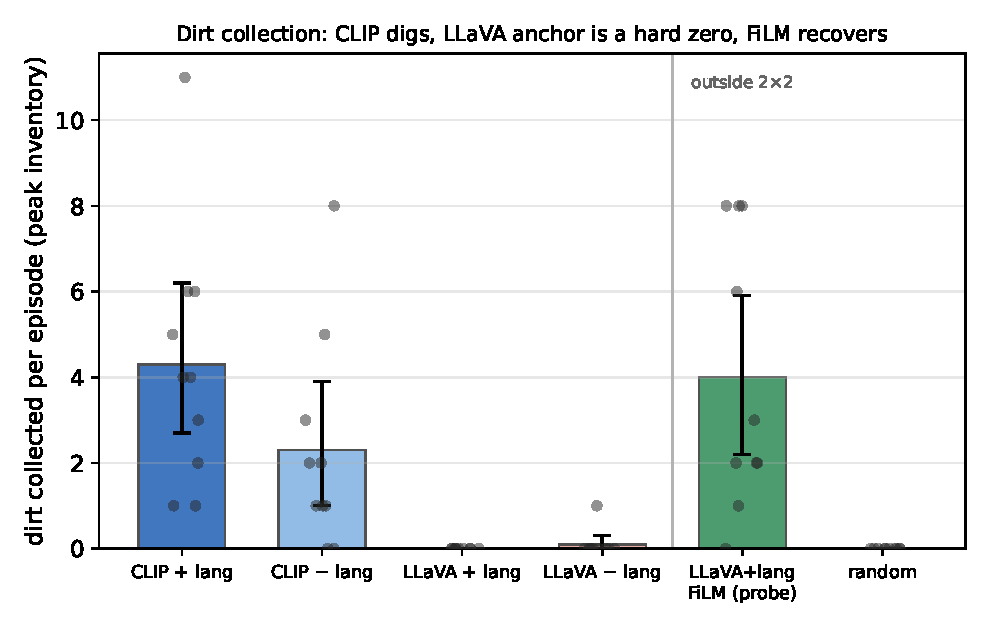
\includegraphics[width=0.92\textwidth]{figures/fig_taskperf.pdf}
\caption{Dirt collected per episode. Bars are means with percentile-bootstrap
$95\%$ intervals; grey dots are the ten individual episodes. The two CLIP cells
dig, the LLaVA anchor cells do not, and the random policy collects nothing. The
FiLM probe (green, right of the divider) lies outside the $2\times2$ and is
discussed in Section~\ref{sec:exp-film}.}
\label{fig:task}
\end{figure}

Task performance separates by backbone, not by language. \textbf{CLIP + lang}
collects $4.3$ dirt per episode and digs in every episode; \textbf{CLIP $-$
lang} collects $2.3$ and digs in eight of ten. Both LLaVA anchor cells are at
the floor: \textbf{LLaVA + lang} returns a hard zero across all ten episodes
(standard deviation $0$), and \textbf{LLaVA $-$ lang} reaches $0.1$ ---
indistinguishable from the random policy's zero. The CLIP--versus--LLaVA gap is
the one task comparison robust to the small sample: a cell that never collects
dirt in ten independent episodes is reliably below a cell that always does. The
within-CLIP gap between the prompt and no-prompt cells ($4.3$ versus $2.3$) is
in the expected direction but \emph{soft}: the two confidence intervals overlap,
so with ten episodes I cannot claim the prompt improves dirt collection; the two
cells are statistically indistinguishable on this metric at this sample size.
This is the honest limit of episode-level metrics at
the sample size the LLaVA backbone makes affordable, and it is why the
conditioning analysis of Section~\ref{sec:exp-cond}, which rests on $10^4$
per-step observations, carries the load-bearing claim.

One caveat on this metric matters, because the dirt count is not a pure measure
of goal pursuit. Comparing the two leftmost columns of Table~\ref{tab:task},
\textbf{CLIP + lang} collects only $0.8$ dirt incidentally in the \emph{chop}
environment but $4.3$ when actually told to collect dirt --- a genuine,
prompt-and-task-driven lift. \textbf{CLIP $-$ lang}, by contrast, digs essentially
the same amount in both environments ($2.5$ versus $2.3$): its dirt comes from
indiscriminately attacking the ground, not from pursuing the goal. Read this way
the task result is sharper than a raw ranking suggests --- it is specifically the
\emph{prompted} CLIP agent whose digging tracks the instruction, the same
conditioning signal of Section~\ref{sec:exp-cond} now visible in an item count
rather than a firing rate --- and it is the prompt-driven lift between
environments, not the absolute count, that cleanly measures task-following.

\section{Offline Frame Metrics and the Offline--Online Gap}
\label{sec:exp-offline}

The rollout results stand in sharp contrast to how the four cells look on the
held-out test frames of Section~\ref{sec:split}. Table~\ref{tab:offline} reports
the offline metrics over $1{,}252{,}328$ test frames per cell. On frames the four
cells are near-indistinguishable: binary-key accuracy is $0.98$ for all four,
\texttt{attack}-$F_1$ is $0.96$, camera bin accuracy is $0.87$ (against a
majority-class, always-still baseline of roughly $78\%$) and camera error is
below half a degree. Even the most behaviourally relevant offline number, the
movement-$F_1$ that selects the checkpoint (Section~\ref{caching}), spans only
$0.368$ to $0.431$ across the four --- and ranks them in an order the rollouts
flatly contradict: \textbf{CLIP $-$ lang} has the \emph{highest} movement-$F_1$
($0.431$) yet collects half the dirt of \textbf{CLIP + lang}, and \textbf{LLaVA
$-$ lang} ($0.368$) sits within $0.04$ of \textbf{CLIP + lang} ($0.407$) yet
collects nothing.

\begin{table}[ht]
\centering
\begin{tabular}{lrrrrr}
\hline
Cell & binary acc & \texttt{attack} $F_1$ & movement $F_1$ & camera acc & camera MAE ($^\circ$) \\
\hline
Exp~2 CLIP + lang    & 0.982 & 0.964 & 0.407 & 0.869 & 0.48 \\
Exp~4 CLIP $-$ lang  & 0.982 & 0.964 & 0.431 & 0.869 & 0.48 \\
Exp~1 LLaVA + lang   & 0.981 & 0.962 & 0.369 & 0.868 & 0.48 \\
Exp~3 LLaVA $-$ lang & 0.981 & 0.962 & 0.368 & 0.868 & 0.49 \\
\hline
\end{tabular}
\caption{Offline frame-level metrics on the held-out test split
($1{,}252{,}328$ frames per cell). Binary accuracy is averaged over the $21$
keys; movement-$F_1$ is the mean $F_1$ over the locomotion keys (the
model-selection criterion of Section~\ref{caching}); camera accuracy is top-1
mu-law bin accuracy on \texttt{camera\_x}. The four cells are a near-tie, and
movement-$F_1$ even ranks CLIP $-$ lang above CLIP + lang --- the reverse of the
rollout ranking.}
\label{tab:offline}
\end{table}

\begin{figure}[ht]
\centering
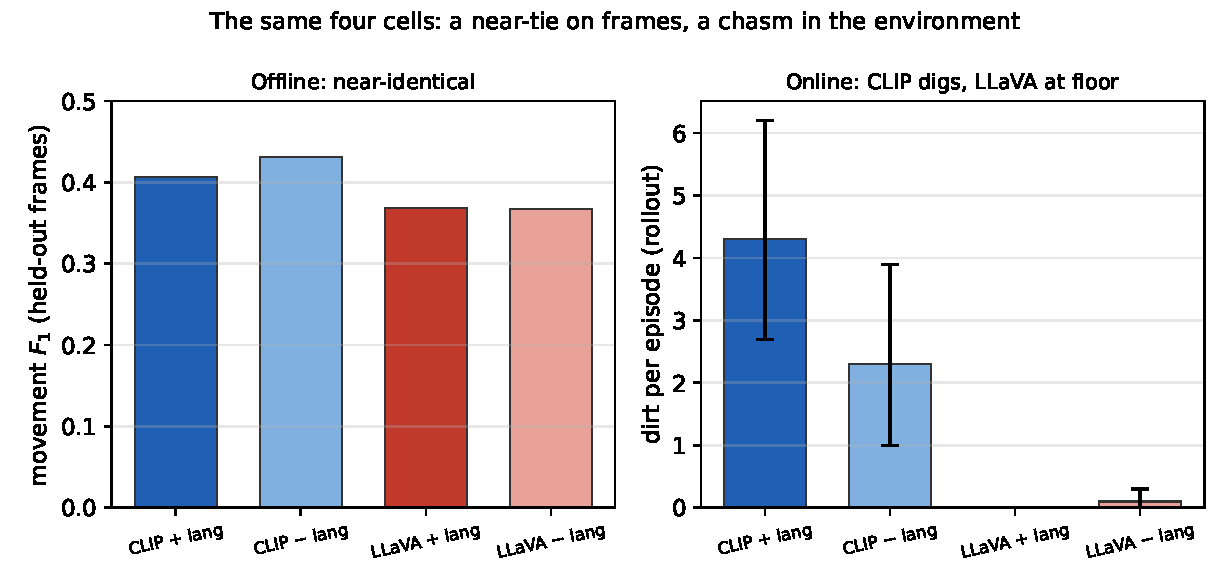
\includegraphics[width=0.95\textwidth]{figures/fig_dissociation.pdf}
\caption{The same four cells, measured two ways. \emph{Left:} movement-$F_1$ on
held-out frames --- a near-tie, with CLIP $-$ lang nominally highest.
\emph{Right:} dirt collected per rollout episode (percentile-bootstrap $95\%$
intervals) --- CLIP digs, both LLaVA cells are at the floor. Frame accuracy does
not predict in-environment behaviour.}
\label{fig:dissociation}
\end{figure}

This offline--online dissociation is the empirical core of the thesis's third
contribution. Held-out frame accuracy --- the metric most imitation-learning work
reports --- would rank these four backbones as interchangeable and would miss the
entire conditioning and task-collection story that appears only once the policy
is closed in the loop. It is a concrete instance of the known weak correlation
between offline action metrics and downstream task success~\cite{kanervisto2020}:
a single mispredicted key every few steps, invisible at the frame level, compounds
over a thousand-step episode into the difference between digging a stack of dirt
and digging nothing. The rollout evaluation is therefore not a costlier
restatement of the frame metrics but a qualitatively different measurement --- and
it is the one that separates the backbones.

\section{Features or Head? A FiLM Probe}
\label{sec:exp-film}

Read on its own, Section~\ref{sec:exp-task} invites the conclusion that the
frozen LLaVA features are useless for control. That conclusion would be too
strong, and a single departure from the $2\times2$ shows why. The LLaVA anchor
feeds the pooled text vector to the head by plain concatenation
(Section~\ref{action_head}); if the head instead conditions on that vector
through feature-wise linear modulation (FiLM), so that the text representation
\emph{scales and shifts} the visual features rather than sitting beside them,
the same frozen LLaVA + lang features that produced a hard zero now collect
$4.0$ dirt per episode at $90\%$ success --- comparable to the best CLIP cell
($4.3$), with the two means well within each other's confidence intervals. The frozen LLaVA
representation therefore \emph{does} carry the information needed to dig; the
anchor's failure is a read-out failure in the head, not an absence of signal in
the features.

Two caveats keep this a probe rather than a result. It is a single architectural
change evaluated on ten episodes, with no matched no-prompt FiLM control, so it
sits deliberately outside the controlled $2\times2$. And it does not recover
conditioning: the FiLM cell still shifts \texttt{attack} by only $+3$~pp between
the empty and on-task prompts, as flat as every other LLaVA cell. A better head
unlocks the \emph{task} signal in the LLaVA features but not a prompt-driven
\emph{conditioning} signal. That a head which multiplicatively gates the visual
features on the text vector still does not condition is itself informative: it
indicates the limit is not head capacity but the pooled text representation, which
does not expose a prompt axis to gate on (Section~\ref{sec:exp-probe}). I return to
the implications of this split in Chapter~\ref{chap:discussion}.

\section{Is the Prompt Represented? A Linear Probe}
\label{sec:exp-probe}

Is the LLaVA conditioning failure a missing signal or an unusable one? A cheap
offline probe narrows it down. On the cached training features I fit a logistic
regression to predict the task --- equivalently, which training prompt was given
--- from the image half of the pooled feature, the text half, and the full
vector, on a balanced $30{,}000$-frame sample (Table~\ref{tab:probe}).

The task is almost perfectly decodable from the pooled LLaVA text half ($99.7\%$),
above the $90.1\%$ reachable from the image half, and it collapses to chance
($50\%$) when the text half is zeroed: the prompt is far from washed out of the
representation. But decodability alone does not make the prompt \emph{usable} for
conditioning, because in the combined training set the two prompts are perfectly
correlated with two visual distributions (forest versus plains) and the pooled
LLaVA text half is image-entangled --- its tokens attend to the frame inside the
decoder. The probe cannot separate a genuine prompt axis from the image content
that leaks into the text positions.

\begin{table}[ht]
\centering
\begin{tabular}{lrrr}
\hline
Cache (probe input) & image & text & full \\
\hline
CLIP + lang ($768/768$)        & 98.3 & 100.0 & 100.0 \\
LLaVA + lang ($4096/4096$)     & 90.1 & 99.7  & 99.3 \\
LLaVA $-$ lang (text zeroed)   & 89.9 & 50.0  & 90.0 \\
\hline
\end{tabular}
\caption{Task-decoding accuracy (\%) of a logistic probe predicting the task
(chop vs dirt, i.e.\ which prompt was given) from each half of the pooled feature
($30{,}000$ balanced frames, $70/30$ split). The LLaVA text half encodes the
prompt almost perfectly, refuting a literally \enquote{washed-out} reading; the
no-prompt control, whose text half is zeroed, drops to chance.}
\label{tab:probe}
\end{table}

Which it is --- a usable axis or a confound --- is settled by the FiLM result.
A head that multiplicatively gates on exactly this text vector
(Section~\ref{sec:exp-film}) is a more expressive way to condition than the
concatenating head, yet it produces no behavioural shift ($+3$~pp). Were the text
half a clean, prompt-isolated axis, such a head would ride it; that it does not
indicates the decodable direction is largely the prompt--image confound rather
than a separable prompt signal. The contrast with CLIP makes this concrete: CLIP's
text encoder is physically separate from its image encoder, so its prompt
embedding is image-independent and moves when, and only when, the prompt changes
--- the axis the head learns to use. The bottleneck for LLaVA is therefore not
that the head is too weak but that its pooled, image-entangled text representation
does not present a prompt axis to act on; the limit sits upstream of the head. A
counterfactual test that changes only the prompt at a fixed frame would measure
the confound directly, and is left to Chapter~\ref{chap:discussion}.

\section{Summary of Findings}
\label{sec:exp-summary}

\begin{itemize}
\item All four cells diverge sharply from a random policy, which fires every key
at $\sim\!10\%$ and collects nothing; the trained agents are genuine policies,
not noise (Figure~\ref{fig:profile}).
\item Language conditioning is a backbone effect. Only CLIP + lang reshapes its
policy with the prompt (\texttt{attack} $-48$~pp, $h=-1.04$); its no-prompt
control and both LLaVA cells stay within the $|h|\le0.17$ noise band
(Table~\ref{tab:conditioning}). The prompt is not missing from LLaVA's features
--- a linear probe recovers the task from its pooled text half at $99.7\%$
(Section~\ref{sec:exp-probe}) --- but it is entangled with the image, and no
head-side lever, the FiLM gate included, turns it into conditioning; the
bottleneck is the pooled representation, not the head.
\item Task performance also separates by backbone: CLIP collects dirt ($4.3$ and
$2.3$ per episode) while both LLaVA anchor cells are at the floor
(Table~\ref{tab:task}). The within-CLIP prompt effect is in the right direction
but not significant at ten episodes; chopping fails for every model. The dirt
count is partly confounded by incidental digging, but it is the prompt-driven
\emph{lift} between environments that is goal-directed, and that lift appears only
for CLIP + lang.
\item Held-out frame metrics do not predict rollout behaviour: all four cells
score within $0.04$ movement-$F_1$ and $0.001$ binary accuracy offline, yet
diverge from $4.3$ to $0$ dirt online --- a direct demonstration that rollout
evaluation measures what frame metrics miss
(Section~\ref{sec:exp-offline}, Figure~\ref{fig:dissociation}).
\item The LLaVA floor is a head limitation, not a feature limitation: a
FiLM-conditioned head lifts dirt collection from zero to $4.0$ per episode,
comparable to the CLIP cells, from the same frozen features, without recovering conditioning
(Section~\ref{sec:exp-film}).
\end{itemize}
